\documentclass[t]{beamer}
\usepackage[portuguese]{babel}
\usepackage[utf8]{inputenc}
\usetheme{Berkeley}
\usecolortheme{seahorse}

\addto\captionsportuguese{
	\renewcommand{\figurename}{Fig.}
	\renewcommand{\tablename}{Tab.}
}

\title{Tratamento de dados}
\subtitle{Como podemos tratar os dados dos dispositivos.}

\AtBeginSection[]
{
	\begin{frame}
	\frametitle{Sumário}
	\tableofcontents[currentsection]
\end{frame}
}

\begin{document}

\frame{\titlepage}

\begin{frame}
\frametitle{Sumário}
\tableofcontents
\end{frame}

\section{Tratamentos}

\begin{frame}{Tratamentos de dados}
Tipos de tratamento
\begin{itemize}
	\item Filtros
	\item Aprendizado
	\item Validação
\end{itemize}
\end{frame}

\begin{frame}{Porque tratar os dados?}
Big Data Vs:
\begin{itemize}
	\item Volume
	\item Velocidade
	\item Variedade
	\item Variabilidade
	\item Veracidade
	\item Validade
	\item Vulnerabilidade
	\item Volatilidade
	\item Visualização
	\item Valor
\end{itemize}
\end{frame}

\section{Filtros}
\begin{frame}{Filtros}
Tipos de filtros
\begin{itemize}
	\item Analógicos
	\item Digitais
	\item Contextuais
\end{itemize}
\end{frame}

\begin{frame}{Filtros}
Filtros comuns
\begin{itemize}
	\item Passa-alta (High Pass Filter)
	\item Passa-baixa (Low Pass Filter)
	\item Passa-banda (Band Pass Filter)
\end{itemize}
\end{frame}

\begin{frame}{Fusão de sensores}
Utilidades
\begin{itemize}
	\item Remover ruídos
	\item Decisões mais inteligentes
	\item Inferir informações
\end{itemize}
\end{frame}

\begin{frame}{Fusão de sensores}
Duplicação de sinal
\begin{figure}
	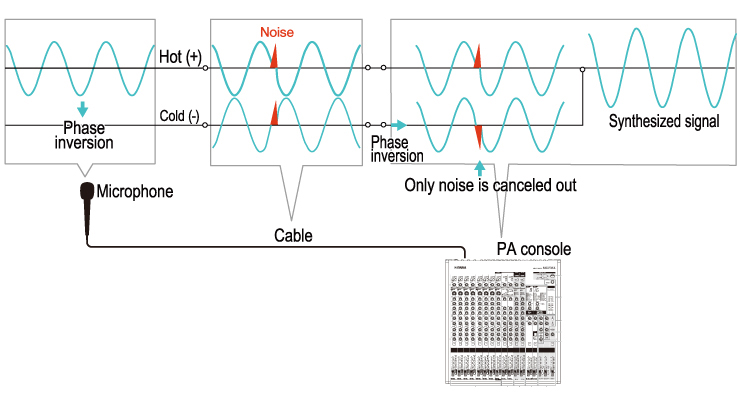
\includegraphics[width=\linewidth]{pa_beginners_cable_ph09}
\end{figure}
\end{frame}

\begin{frame}{Fusão de sensores}
Sensores magnéticos
\begin{figure}
	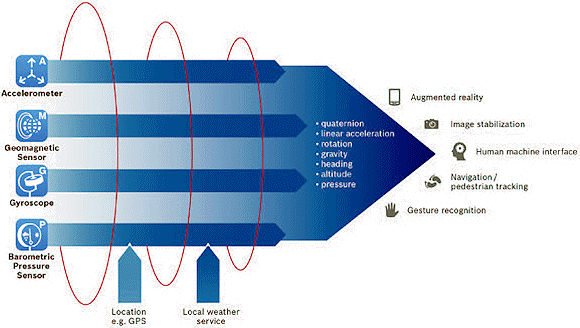
\includegraphics[width=\linewidth]{sensorfusion}
\end{figure}
\end{frame}

\begin{frame}{Fusão de sensores}
Exemplo com radares
\begin{figure}
	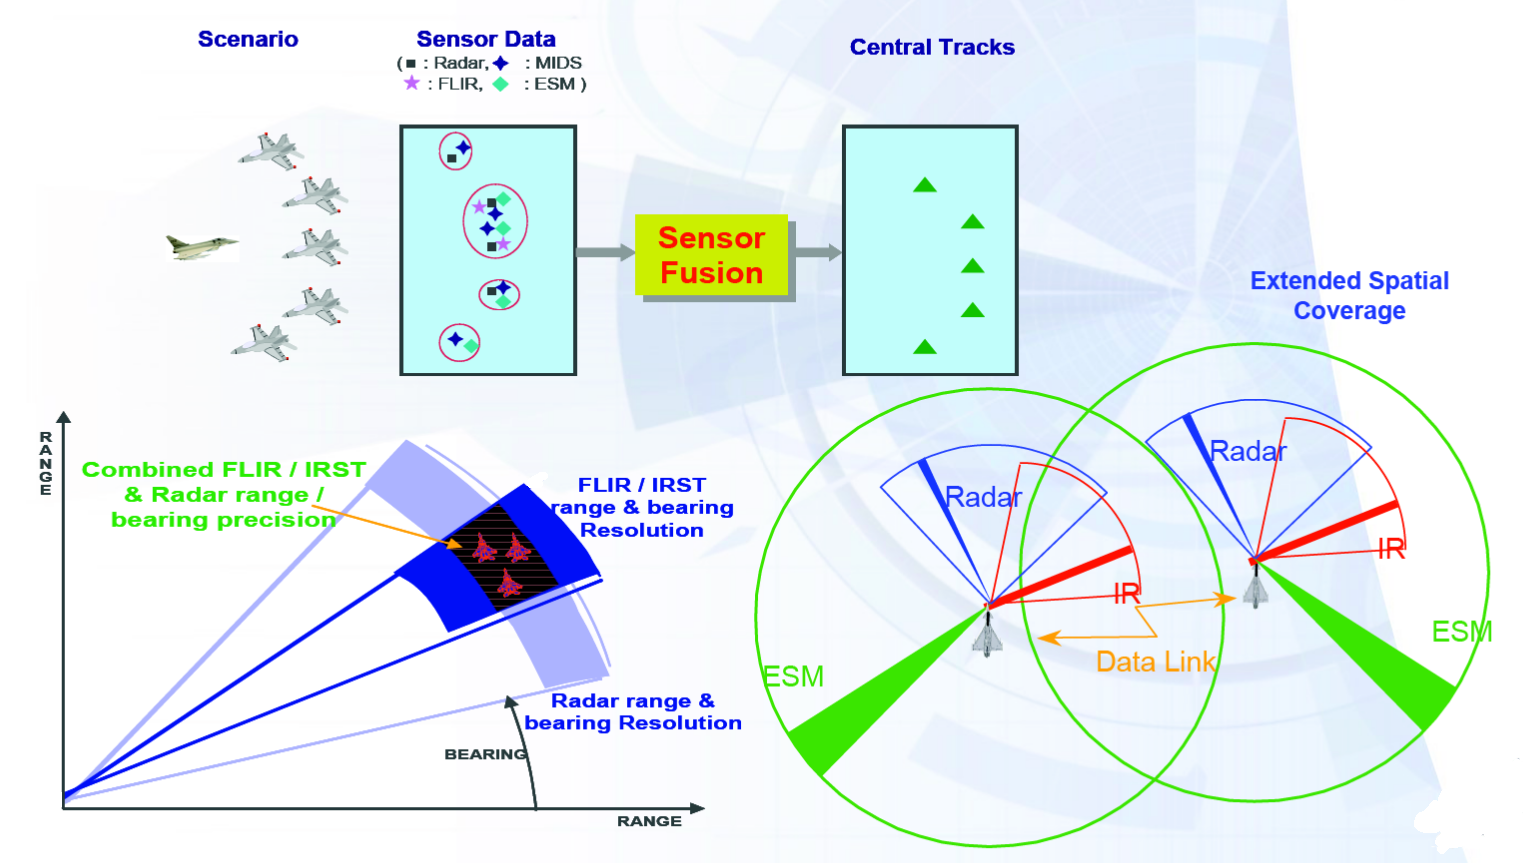
\includegraphics[width=\linewidth]{Eurofighter_sensor_fusion}
\end{figure}
\end{frame}

\begin{frame}{Fusão de sensores}
Carro autônomo
\begin{figure}
	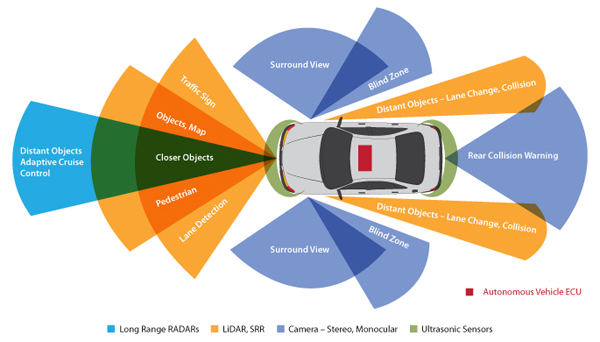
\includegraphics[width=\linewidth]{5_TataElxsiAutonomaisensorfusionschematic}
\end{figure}
\end{frame}

\begin{frame}{Fusão de sensores}
Carro autônomo
\begin{figure}
	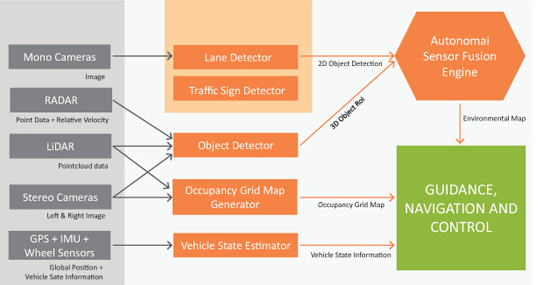
\includegraphics[width=\linewidth]{5_TataElxsiAutonomaiperceptionschematic}
\end{figure}
\end{frame}

\section{Aprendizado de Máquina}


\begin{frame}{Aprendizado de máquina}
Por que?!
\begin{itemize}
	\item Muitos dados
	\item Segurança para informações e sistemas
	\item Aumentar poder computacional
	\item Consumo eficiente de recursos e energia
	\item Crescimento constante de algoritmos e teorias
\end{itemize}
\end{frame}

\begin{frame}{Aprendizado de máquina}
\begin{figure}
	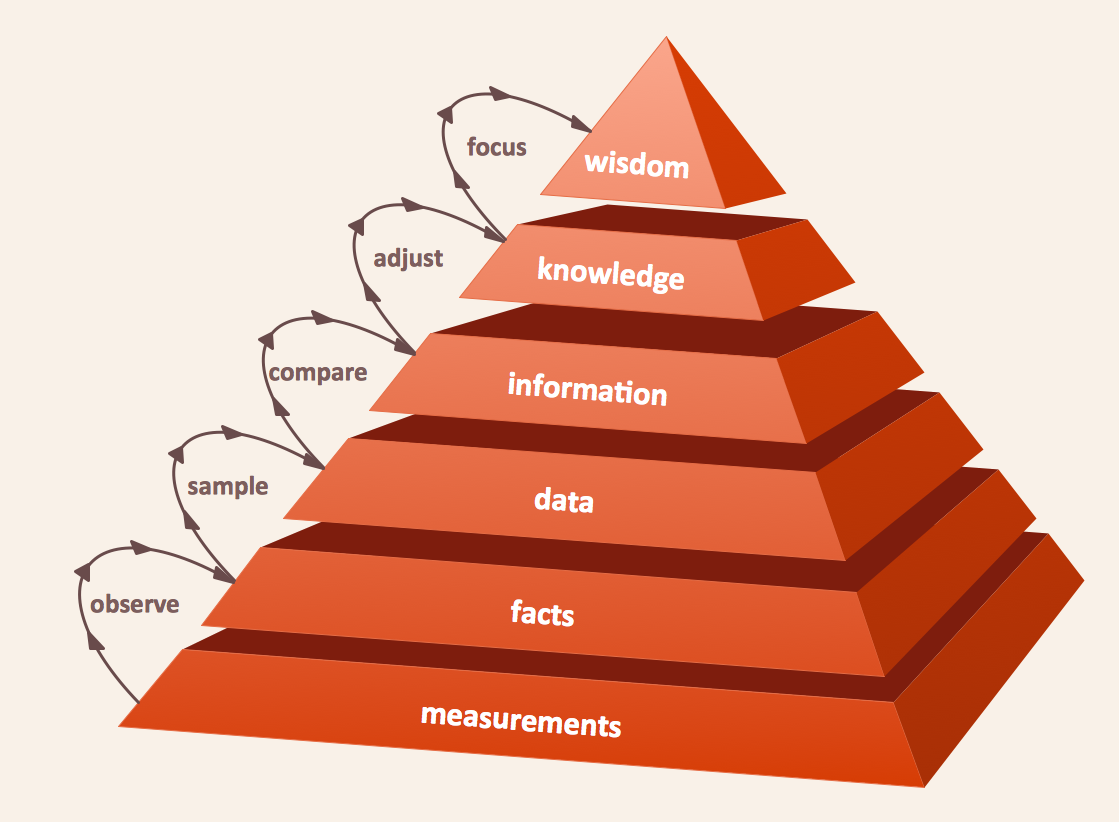
\includegraphics[width=\linewidth]{PYRAMID-DIKW-hierarchy-3d-pyramid}
\end{figure}
\end{frame}

\begin{frame}{Aprendizado de máquina}
\begin{figure}
	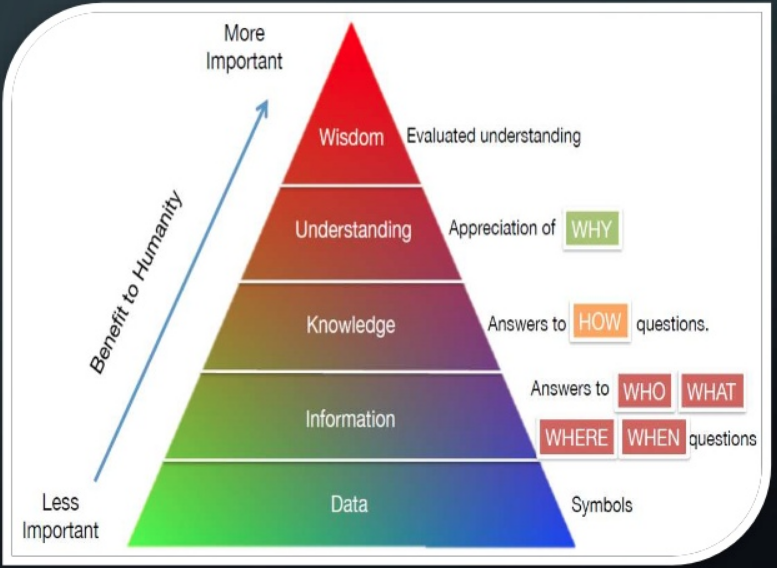
\includegraphics[width=\linewidth]{beneficiosdaanalisedosdados}
\end{figure}
\end{frame}

\begin{frame}{Aprendizado de máquina}
\begin{figure}
	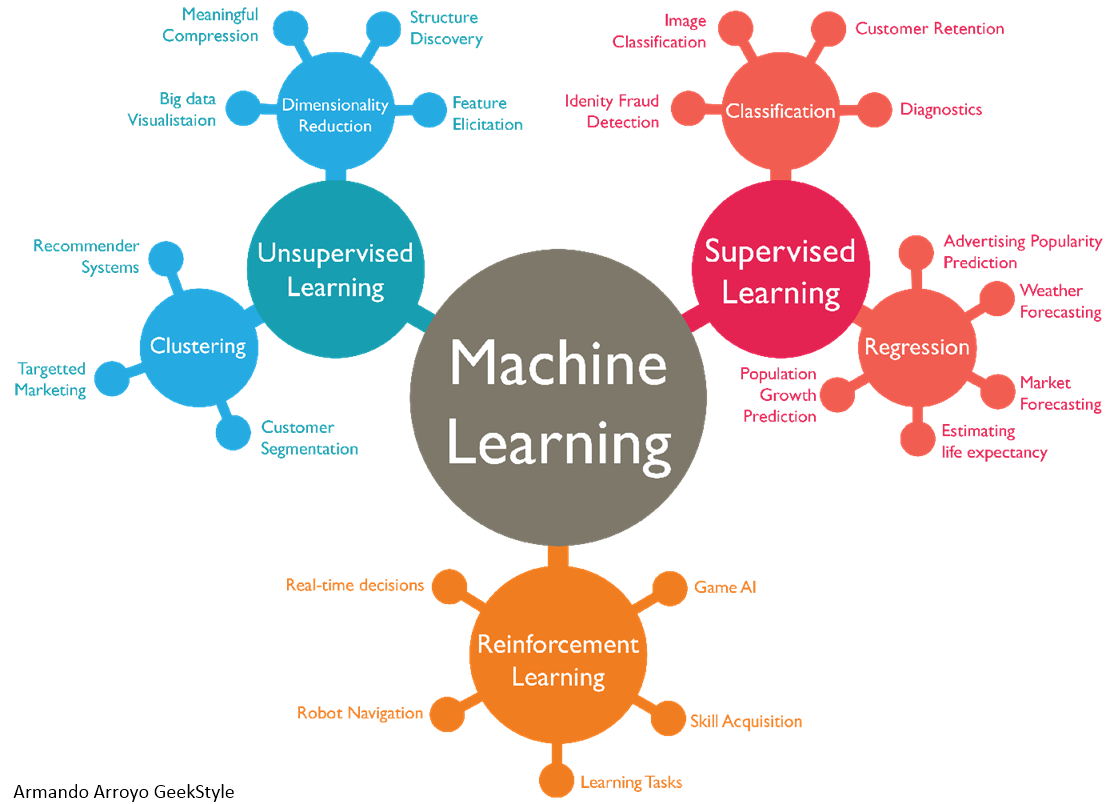
\includegraphics[width=\linewidth]{machinelearning}
\end{figure}
\end{frame}



\frame{\titlepage}

\end{document}
